%*----------- SLIDE -------------------------------------------------------------
\begin{frame}[c]{Contradições no discurso de Bolsonaro}
    %\transboxin[duration=1,direction=30]


    \begin{figure}
        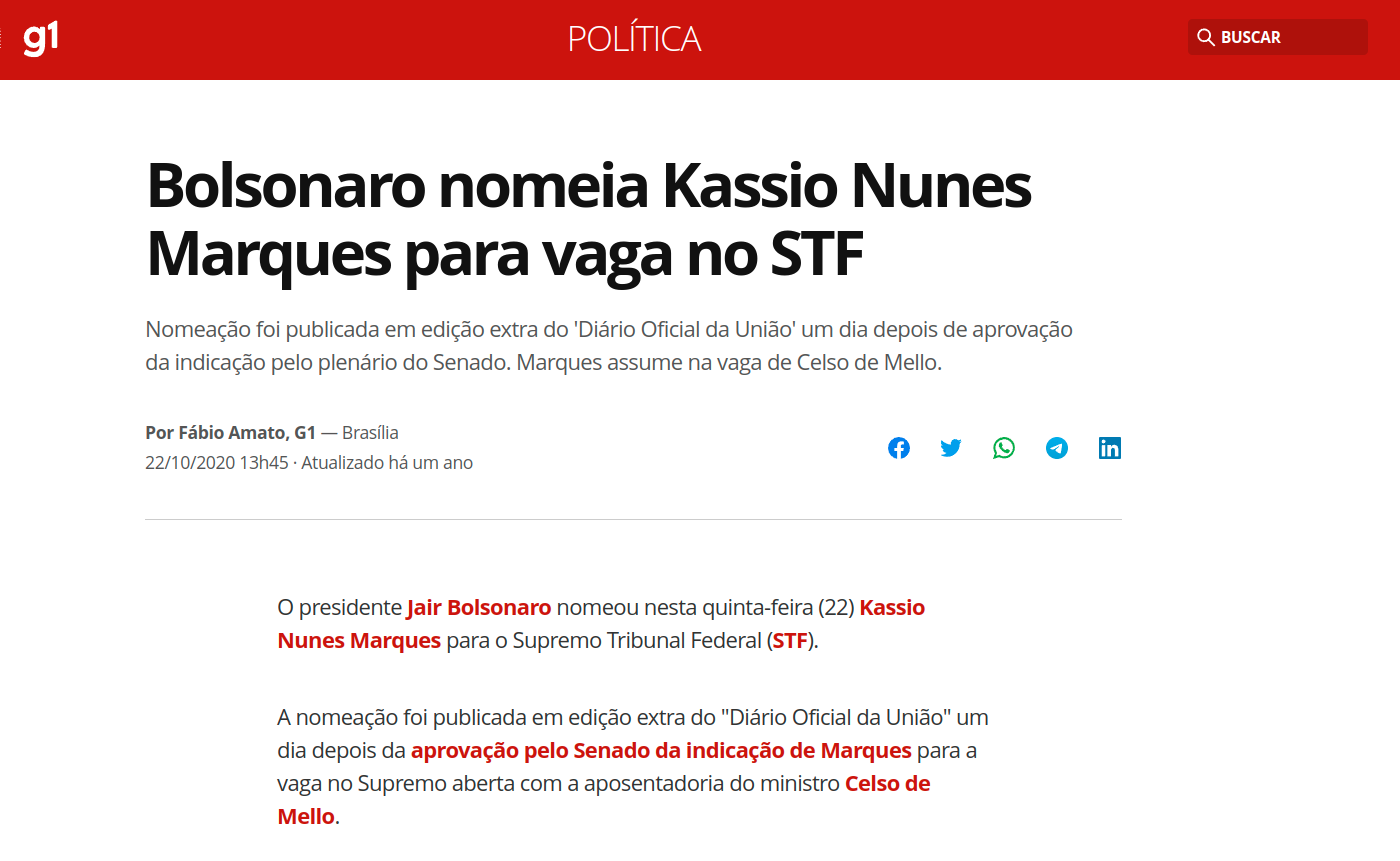
\includegraphics[trim = 0 20 0 20, clip, width=0.8\textwidth]{kassio-stf.png}
        \caption{\cite{Amato_fabio}}
    \end{figure}

%*----------- notes
    \note[item]{Notes can help you to remember important information. Turn on the notes option.}
\end{frame}
%-
%*----------- SLIDE -------------------------------------------------------------
\begin{frame}[t]{Ligações com o PT}


    \begin{figure}
        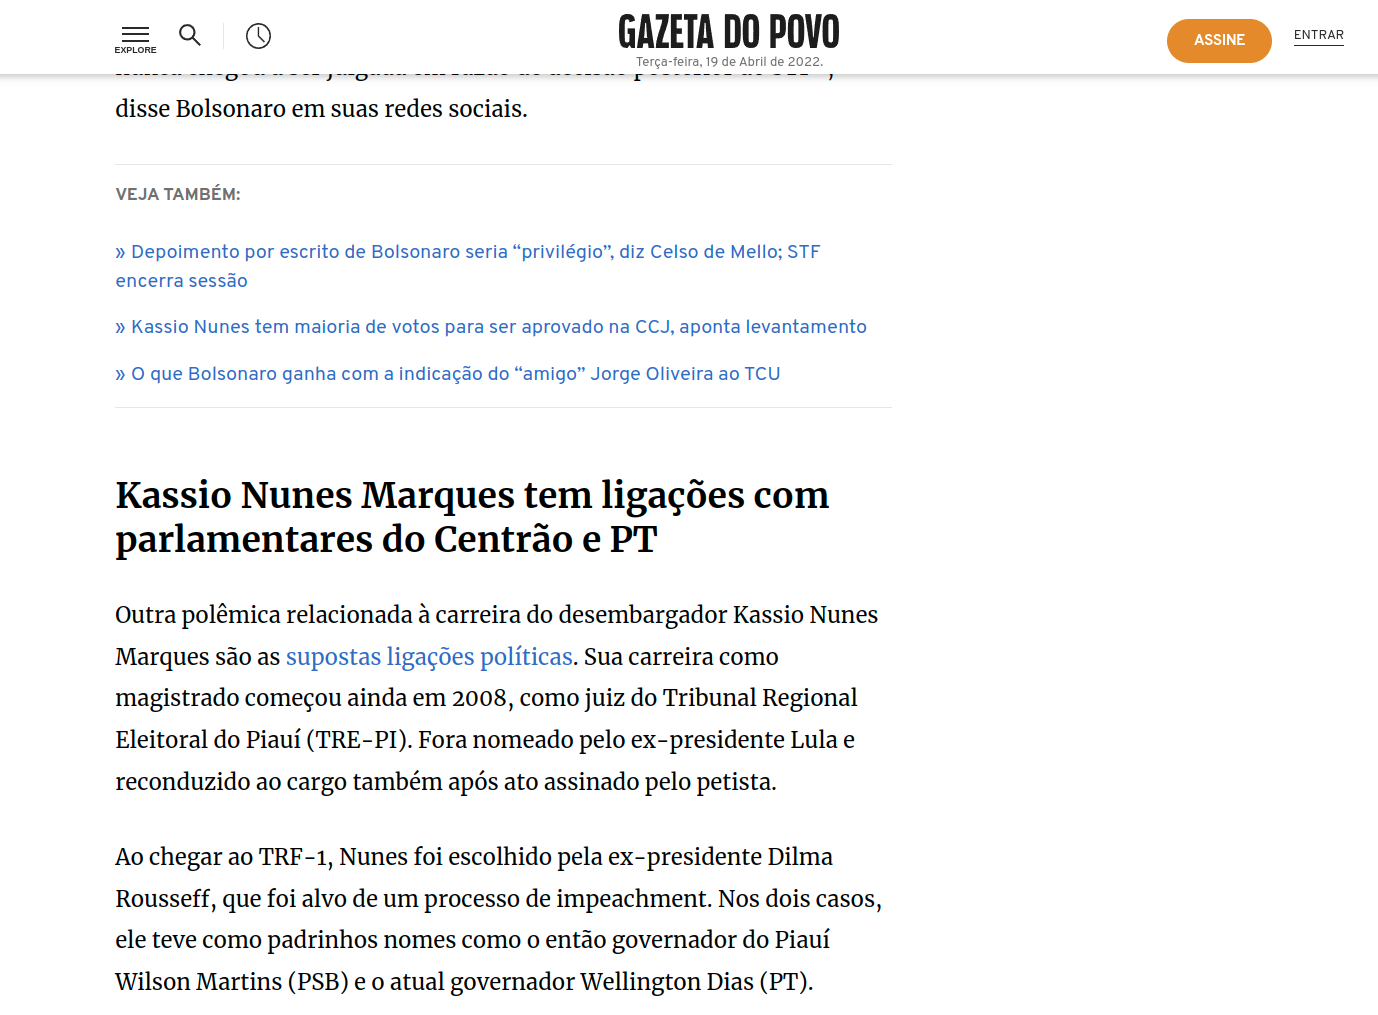
\includegraphics[trim = 0 20 0 20, clip, width=0.8\textwidth]{kassio-pt.png}
        \caption{\cite{Lima_wilson}}
    \end{figure}

%*----------- notes
    \note[item]{Notes can help you to remember important information. Turn on the notes option.}
\end{frame}
%-
%*----------- SLIDE -------------------------------------------------------------
\begin{frame}[c]{Augusto Aras na PGR}
    \begin{figure}
        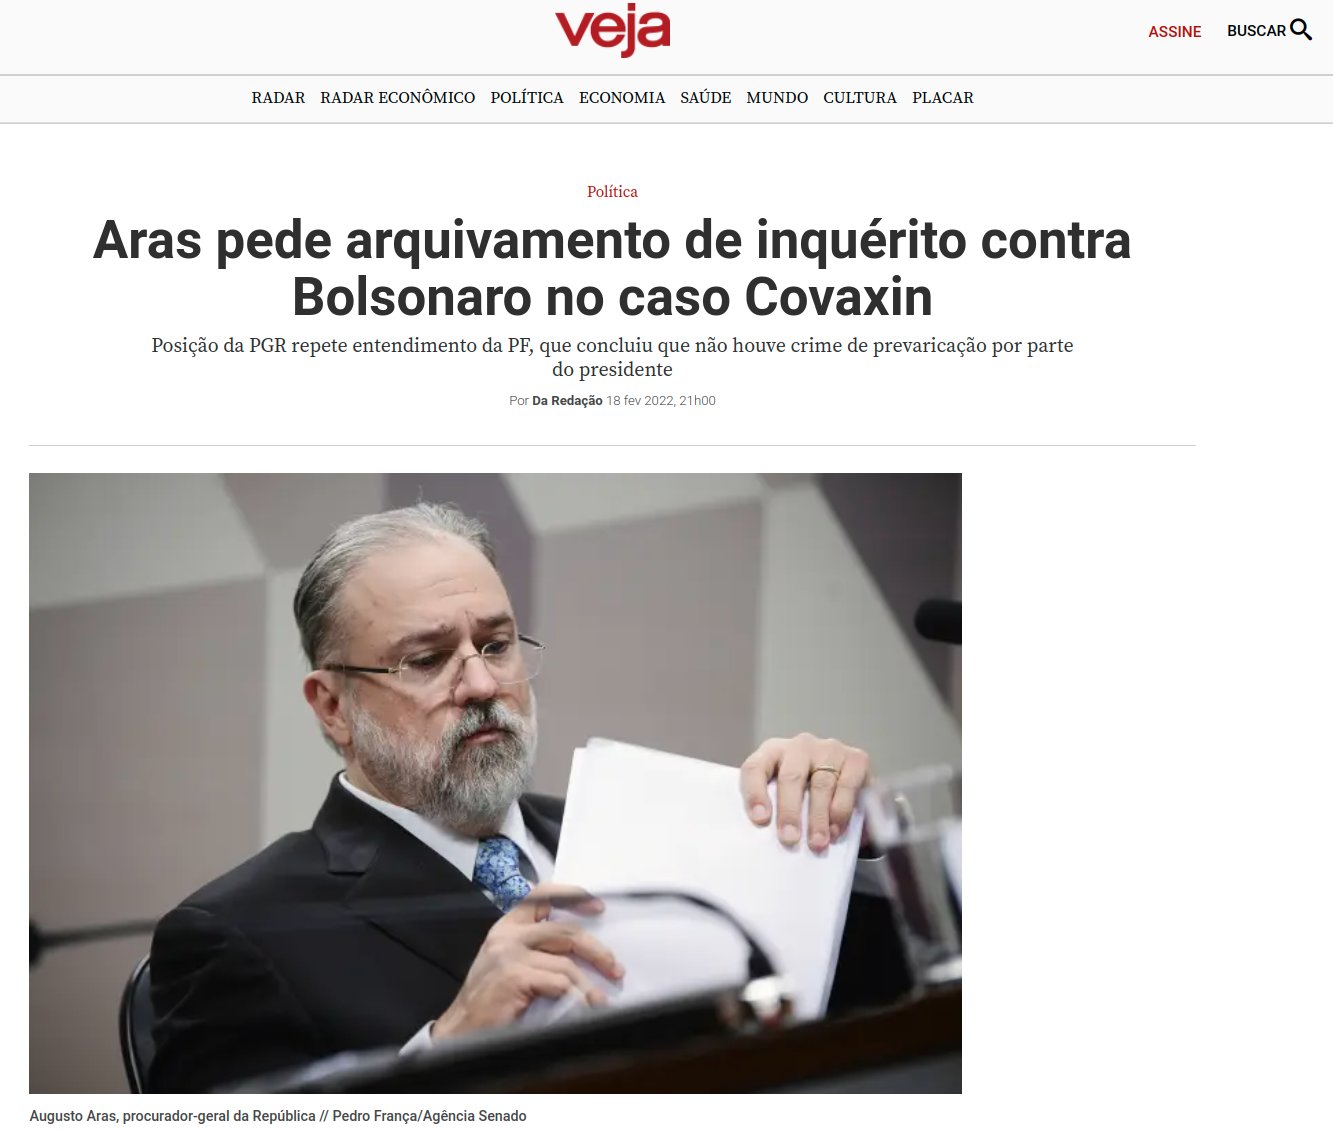
\includegraphics[trim = 0 20 0 10, clip, width=0.8\textwidth]{Aras.png}
        \caption{\cite{Da_redacao}}
    \end{figure}
%*----------- notes
    \note[item]{Notes can help you to remember important information. Turn on the notes option.}
\end{frame}
%*----------- SLIDE -------------------------------------------------------------
\begin{frame}[c]{Lava Toga}
    \begin{figure}
        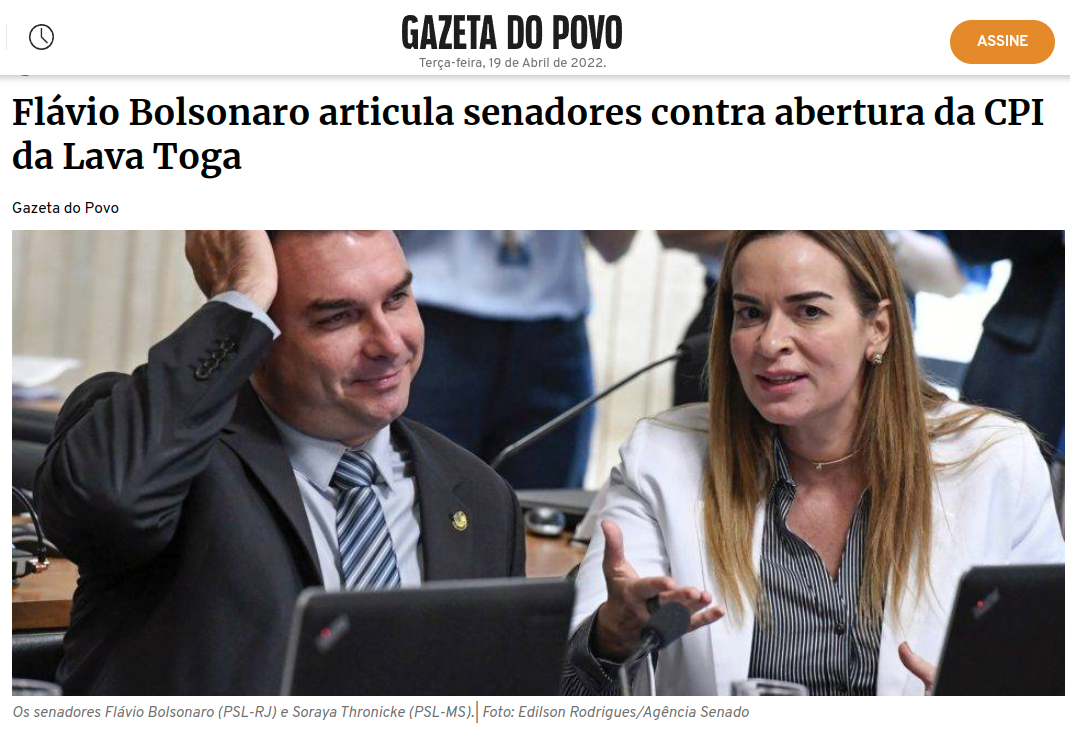
\includegraphics[trim = 0 20 0 10, clip, width=0.8\textwidth]{flavio-lavatoga.png}
        \caption{\cite{Rodrigues_edilson}}
    \end{figure}
%*----------- notes
    \note[item]{Notes can help you to remember important information. Turn on the notes option.}
\end{frame}